%***********************************************************************
\subsection{Calibration Evaluation}\label{sub:bc_calibration_evaluation}
%***********************************************************************

% Opening Paragraph
The implication of the model parameters posterior uncertainty on the prediction is investigated by propagating the uncertainty through \gls[hyper=false]{trace} simulations of test No. $216$ (the calibration data) as well as the other five \gls[hyper=false]{feba} tests.
Samples of size $1'000$ are randomly picked directly from the joint posterior samples and are used to execute \gls[hyper=false]{trace} simulations.
Furthermore, the uncertainties related to the boundary conditions ($4$ additional parameters, namely \texttt{breakP}, \texttt{fillV}, \texttt{fillT}, and \texttt{pwr}) are also propagated alongside the posterior samples from each calibration scheme.  
Finally, for comparison purpose and for selected calibration schemes, the uncertainty propagation is also conducted without taking into account the correlation structure of the model parameters posterior uncertainties.
In other words, only the information from the posterior univariate marginals is used for the propagation and the parameters are considered independent of each other.

% Explaining the figure
Figs.~\ref{fig:ch5_plot_trace_uq_post_all_disc_tc_216}, \ref{fig:ch5_plot_trace_uq_post_all_disc_dp_216}, and~\ref{fig:ch5_plot_trace_uq_post_all_disc_co_216} show the propagation of the uncertainties for the clad temperature ($TC$), the pressure drop ($DP$), and the liquid carryover ($CO$) outputs, respectively.
The model parameters posterior uncertainties used in these figures are the ones obtained from the calibration scheme with model bias term and considering all types of output (i.e., \texttt{w/ Bias} in Table~\ref{tab:ch5_calibration_schemes}). 
The uncertainty bands correspond to the symmetric $95\%$ probability of the output uncertainties, i.e., the area between $2.5$-th and $97.5$-th percentiles of the outputs at each time step.
The dark gray band corresponds to the model parameters prior uncertainties propagation, while the two lighter bands correspond to the posterior uncertainties.
Two posterior uncertainties propagation results are presented, one (the lighter band) takes into account correlation structure of the posterior samples while the other one does not (i.e., independent samples).
This color convention will be used in all the other presentations of the uncertainty propagation results.
Finally, solid lines, dashed lines, and crosses correspond to the simulation with the nominal parameters values, the median of the posterior runs, and the experimental data, respectively.

% FEBA Test No. 216 Posterior w/ bias term Uncertainty Propagation, TC
\begin{sidewaysfigure}
	\centering
	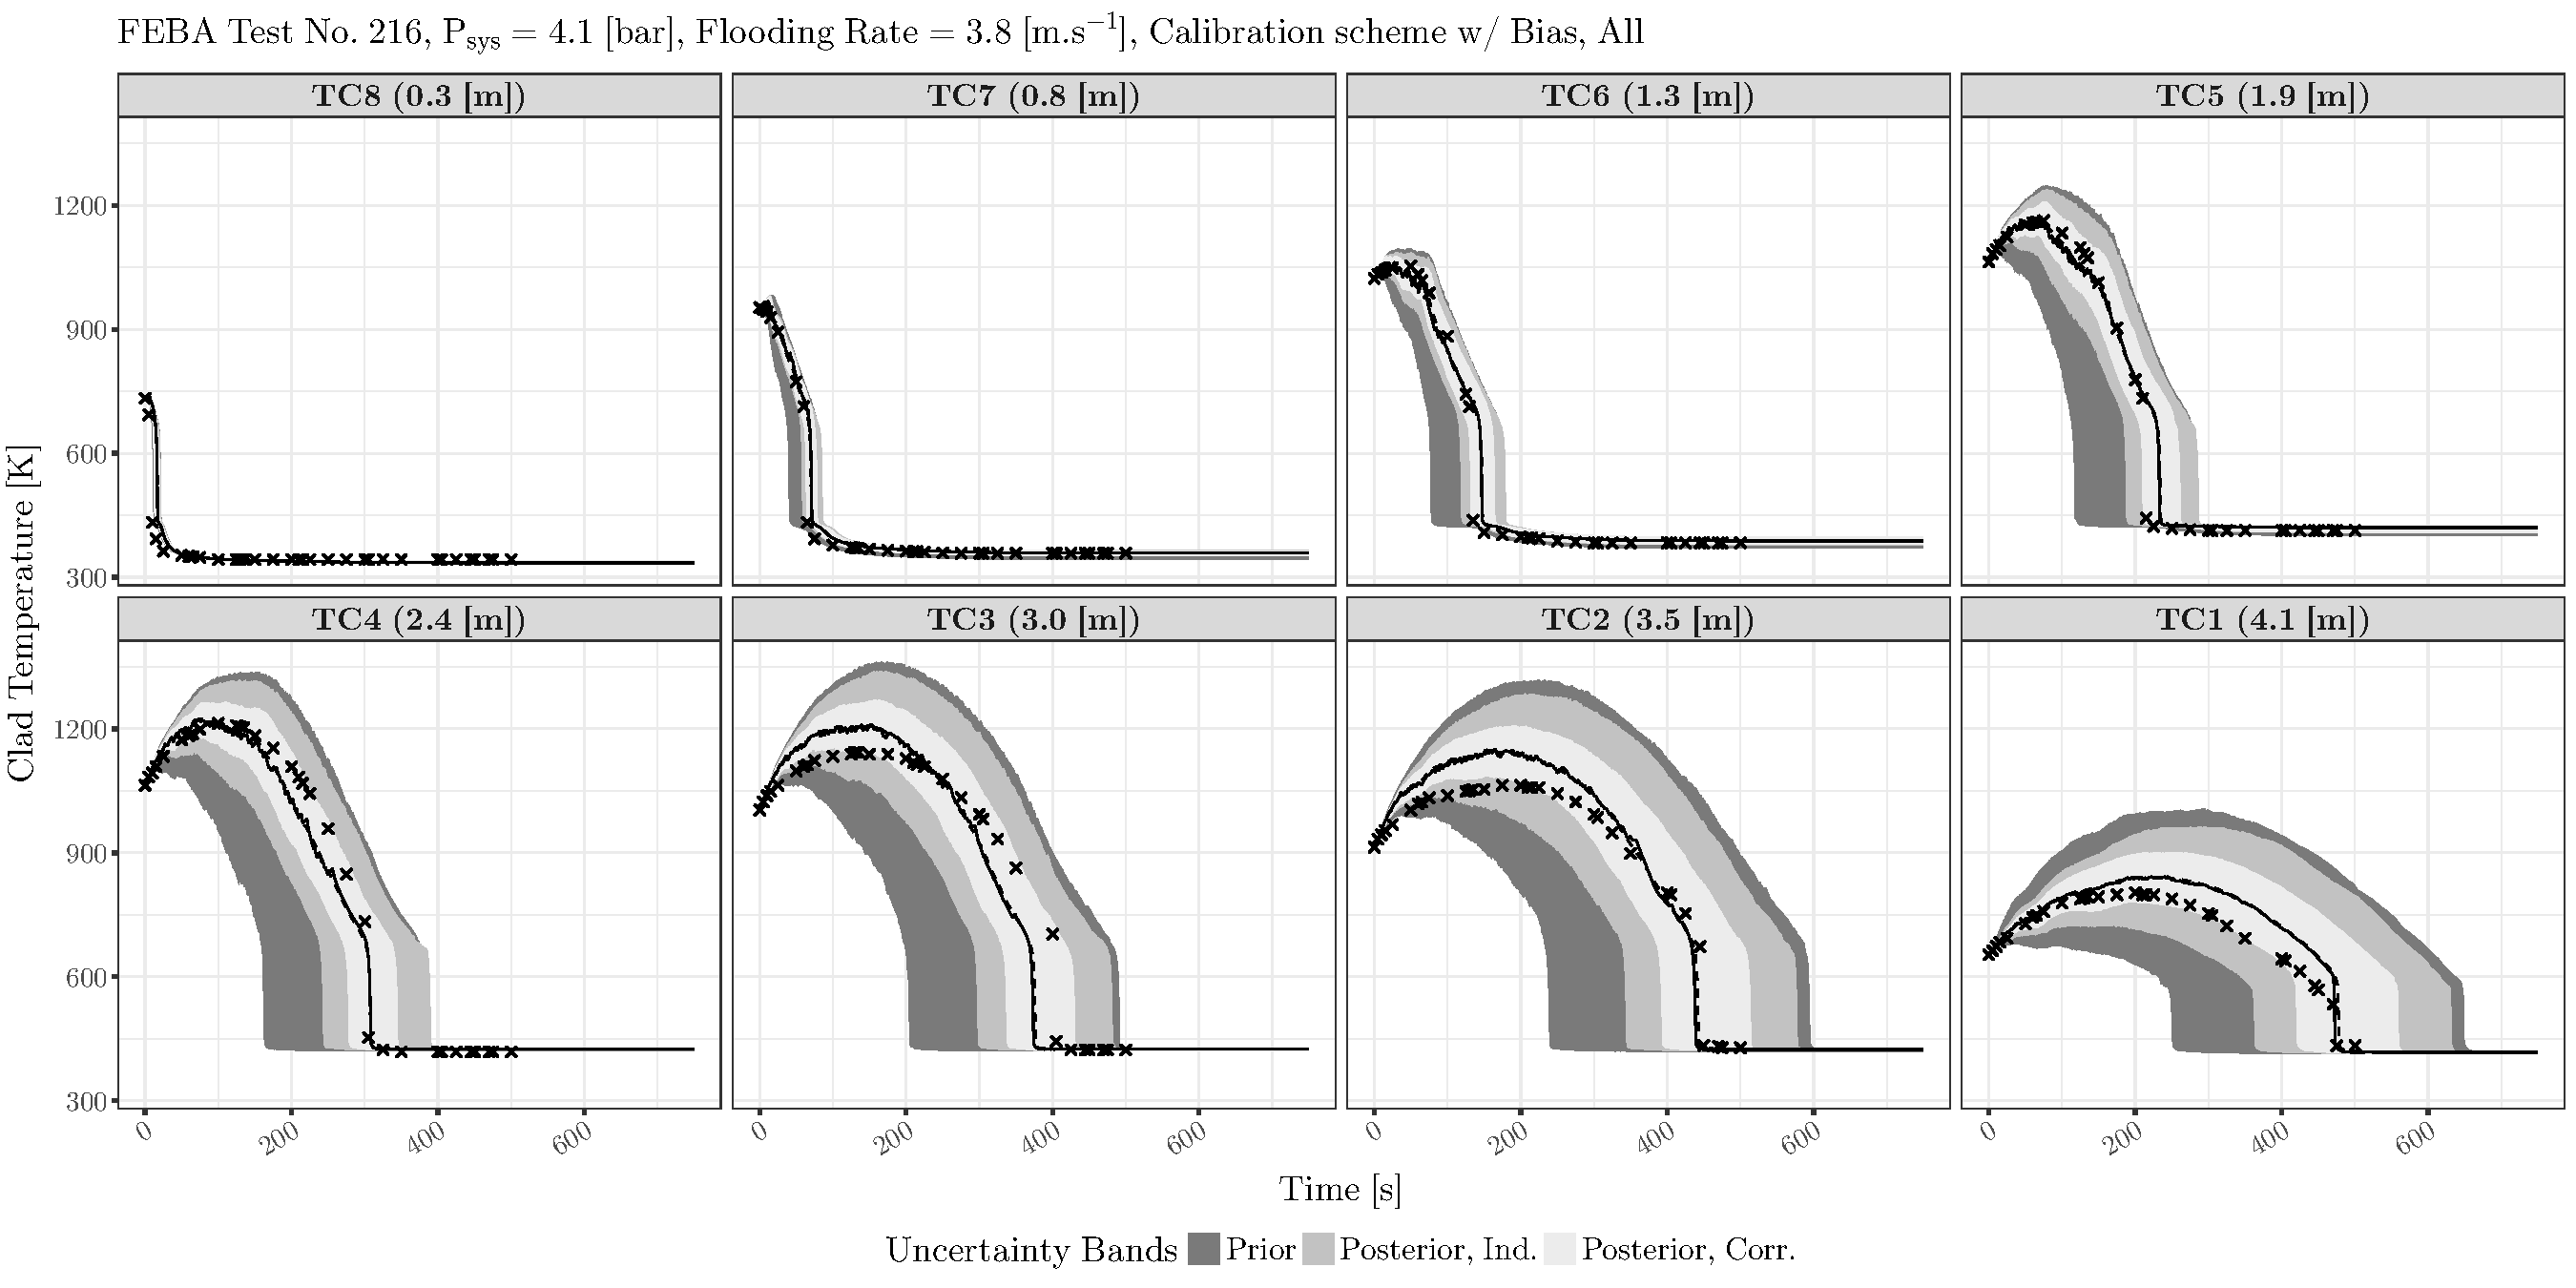
\includegraphics[width=0.90\textwidth]{../figures/chapter5/figures/plotTraceUQPosteriorAllDiscCenteredTC216}
		\captionof{figure}[Posterior uncertainty propagation of FEBA Test No. $216$ for the cladding temperature output ($TC$). Calibration with model bias term and considering all types of output.]{Uncertainty propagation of the parameters uncertainty of \gls[hyper=false]{feba} Test No. $216$ for the cladding temperature output ($TC$) at different axial locations. The uncertainty bands refer to the symmetric $95\%$ probabilities. Solid lines, dashed lines, and crosses indicate the simulation with the nominal parameters values, the median of the posterior, and the experimental data, respectively. The posterior samples are from the calibration with model bias term and considering all types of output.}
	\label{fig:ch5_plot_trace_uq_post_all_disc_tc_216}
\end{sidewaysfigure}

% Explaining the figure, TC
Fig.~\ref{fig:ch5_plot_trace_uq_post_all_disc_tc_216} shows the uncertainty propagation for the time-dependent $TC$ outputs at all axial levels with the posterior samples correspond to the calibration scheme \texttt{w/ Bias, All}.
As can be seen the posterior uncertainties of the clad temperature prediction are narrower as compared to the prior uncertainties across all axial elevation and at all time points.
All uncertainty bands, however, shows similar behavior regarding their inflation going from the bottom part of the assembly to the top of the assembly, and from the start of the transient to the time of quenching.
Furthermore, the median of the posterior predictions (dashed lines) coincides almost perfectly with the prediction of the nominal \gls[hyper=false]{trace} run (solid lines).

A comparison between the bands of correlated posterior samples and of independent posterior samples shows that the prediction uncertainties obtained using the correlated samples are much narrower and, at times, the experimental data points fall outside the uncertainty band.
However, the shape of the band looks consistent with the nominal run.
For instance, looking at the panel of $TC2$ in Fig.~\ref{fig:ch5_plot_trace_uq_post_all_disc_tc_216},
it can inferred that for the simulation to envelop the experimental data points in the early transient, it will also result in a reflood curve that increase the discrepancy even more in the later phase of the transient, especially near the time of quenching.
In other words, there is a certain ``rigidity'' associated with the \gls[hyper=false]{trace} reflood curve that cannot be arbitrarily bend.

On the other hand, not considering the correlation between model parameters in the posterior samples results in inflated uncertainties in the clad temperature prediction.
While the lower uncertainty bound for the independent samples is much narrower than that of the prior, the upper uncertainty bound is closer to the upper uncertainty bound than that of the prior.

% FEBA Test No. 216 Posterior w/ bias term Uncertainty Propagation, DP
Fig.~\ref{fig:ch5_plot_trace_uq_post_all_disc_dp_216} shows the uncertainty propagation for the time-dependent $DP$ outputs for each of the axial segments.
The posterior samples correspond to the calibration scheme \texttt{w/ Bias, All}.
Once again the posterior uncertainties propagation result in narrower uncertainty bands as compared to that with the prior across all axial segments and all time points.
However, the difference between taking and not taking into account correlation between model parameters is less striking for this type of output.
Moreover, all uncertainty bands cover most of the experimental data.
\bigfigure[pos=tbhp,
           opt={width=1.0\textwidth},
           label={fig:ch5_plot_trace_uq_post_all_disc_dp_216},
           shortcaption={Posterior uncertainty propagation of FEBA Test No. $216$ for the pressure drop output ($DP$). Calibration with model bias term and considering all types of output.}]
{../figures/chapter5/figures/plotTraceUQPosteriorAllDiscCenteredDP216}
{Uncertainty propagation of the parameters uncertainty of \gls[hyper=false]{feba} Test No. $216$ for the pressure drop output ($DP$) at different axial segments. The uncertainty bands refer to the symmetric $95\%$ probabilities. Solid lines, dashed lines, and crosses indicate the simulation with the nominal parameters values, the median of the posterior, and the experimental data, respectively. The posterior samples are from the calibration scheme \texttt{w/ Bias, All}.}

% FEBA Test No. 216 Posterior w/ bias term Uncertainty Propagation, CO
Fig.~\ref{fig:ch5_plot_trace_uq_post_all_disc_co_216} shows the propagation for the time-dependent $CO$ output up to the saturation of the measurement tank at $10 [kg]$ with the posterior samples correspond to the calibration scheme \texttt{w/ Bias, All}.
Unlike the previous two types of output, the nominal \gls[hyper=false]{trace} prediction exhibits large bias compared to the experimental data.
While the large prior uncertainty manages to cover the experimental data points, all of the points fall outside the posterior uncertainty bounds both with and without taking into account correlation among parameters.
As the calibration scheme \texttt{w/ Bias, All} simultaneously takes into account the three types of output, and considering the results of uncertainty propagation for the two other outputs, it can be inferred that this failure to cover the experimental data points is off-set by the more consistent bands for the other two outputs.
\begin{figure}[!bth]
    \centering
    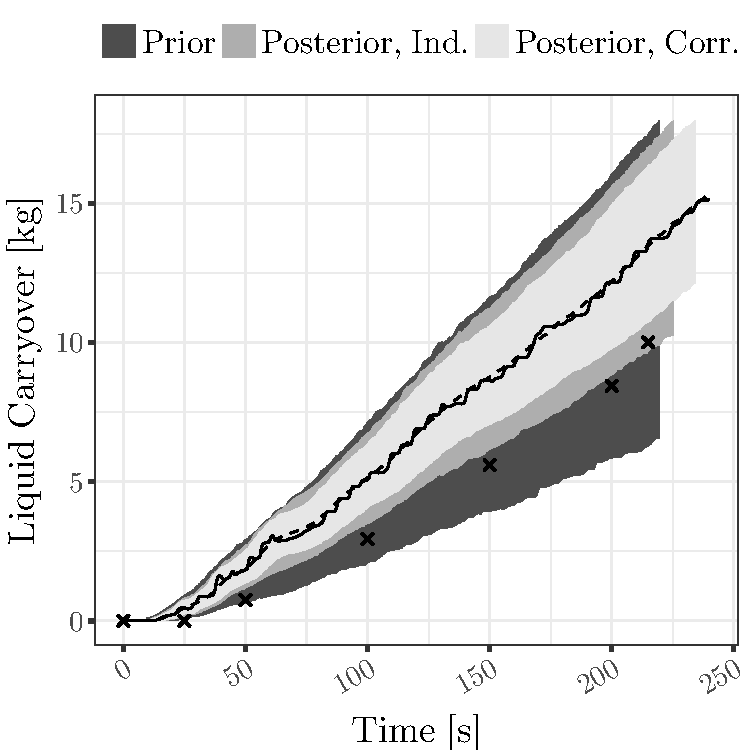
\includegraphics[width=0.5\textwidth]{../figures/chapter5/figures/plotTraceUQPosteriorAllDiscCenteredCO216}
    \caption[Posterior uncertainty propagation of FEBA Test No. $216$ for the liquid carryover output ($CO$). Calibration with model bias term and considering all types of output.]{Uncertainty propagation of the parameters uncertainty of \gls[hyper=false]{feba} Test No. $216$ for the liquid carryover output ($CO$). The uncertainty bands refer to the symmetric $95\%$ probabilities. Solid lines, dashed lines, and crosses indicate the simulation with the nominal parameters values, the median of the posterior, and the experimental data, respectively. The posterior samples are from the calibration scheme \texttt{w/ Bias}.}
    \label{fig:ch5_plot_trace_uq_post_all_disc_co_216}
\end{figure}

% Calibration Score vs Informativeness, how to read the plot
Instead of showing similar plots of the uncertainty propagation for the results of other calibration schemes and for all the other \gls[hyper=false]{feba} tests, Fig.~\ref{fig:ch5_plot_calib_info} summarizes the propagation for the other cases in a single plot using the concept of \emph{calibration score} and \emph{informativeness} previously explained (see Section~\ref{sub:bc_simulation_experiment} and Appendix~\ref{app:calib_info}).
\clearpage
\begin{sidewaysfigure}
	\centering
	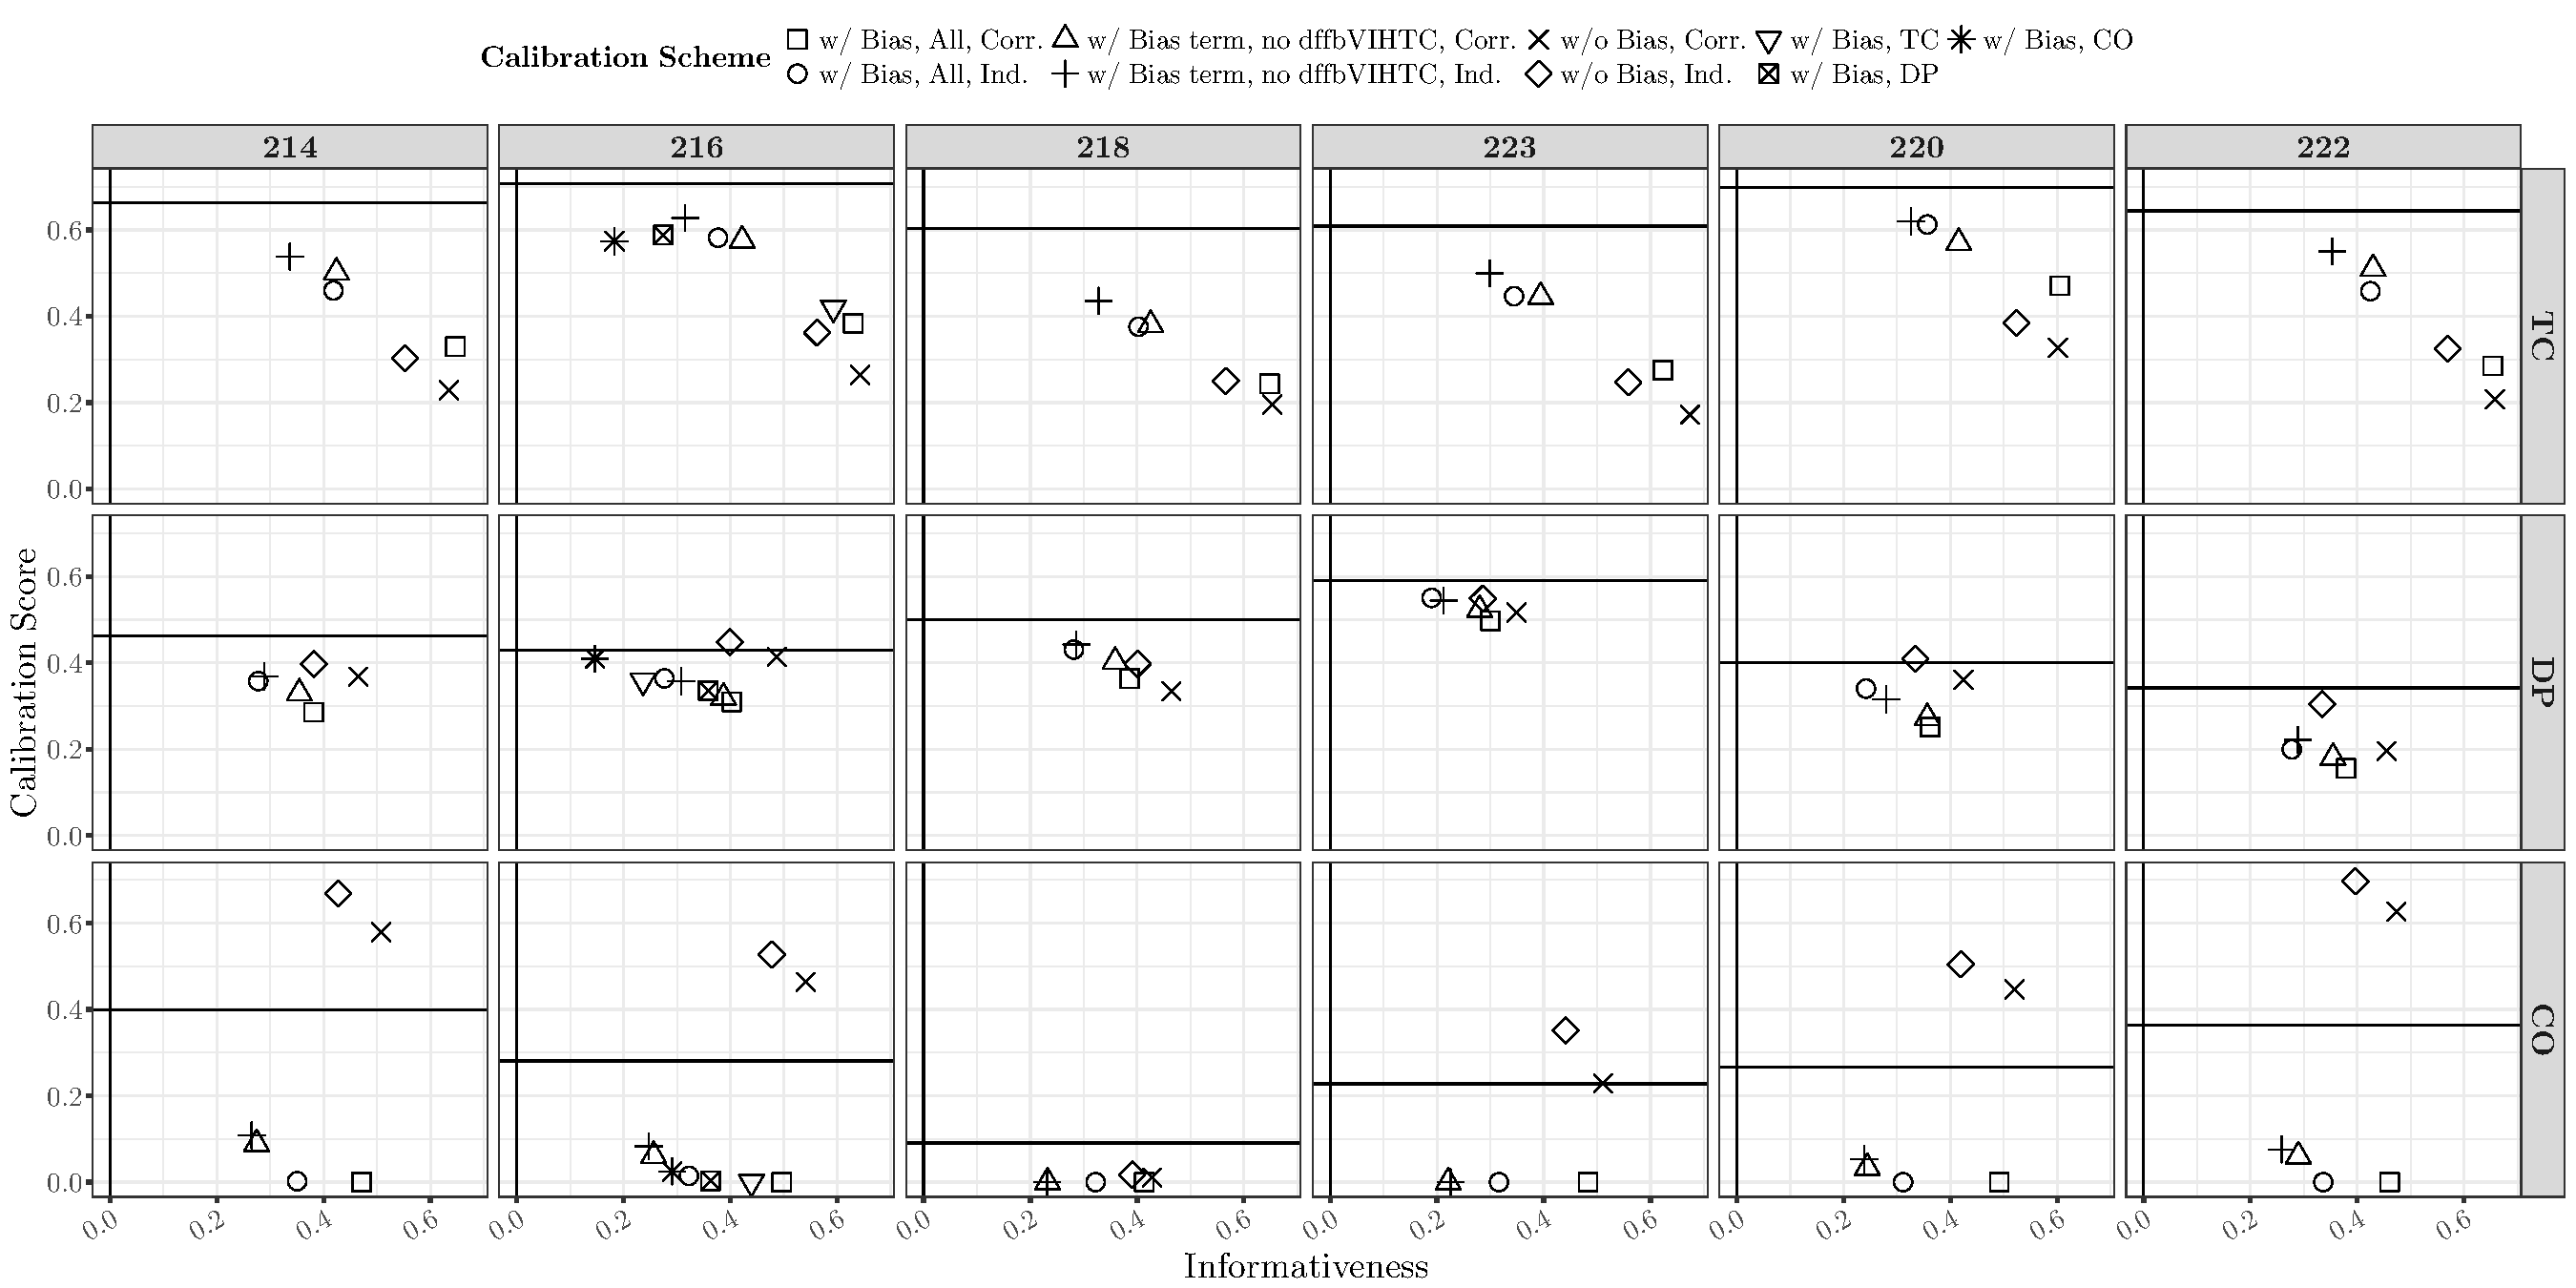
\includegraphics[width=0.95\textwidth]{../figures/chapter5/figures/plotCalibInfo}
		\captionof{figure}[Calibration score vs. Informativeness for different posterior samples propagated on all the FEBA tests.]{Calibration score vs. Informativeness for different posterior samples propagated on all the \gls[hyper=false]{feba} tests. Vertical lines indicate the informativeness of the prior uncertainty (defined as $0$) while the horizontal lines indicate the initial Calibration score (i.e., that of the prior).}
	\label{fig:ch5_plot_calib_info}
\end{sidewaysfigure}
\clearpage


% Comparing Results, additional output

% Comparing Results, calibration scheme

% Comparing Results, correlated vs independent posterior samples

% Comparing Results, between FEBA Tests
